\documentclass[10pt,a4paper,fleqn]{article}
\usepackage[utf8]{inputenc}
\usepackage{amsmath}
\usepackage{amsfonts}
\usepackage{amssymb}
\usepackage{fullpage}
\usepackage{amsthm}
\usepackage{graphicx}

\newcommand{\example}[1]{\textbf{Example}: \emph{#1}}
\newcommand{\justification}[1]{\text{[\textbf{#1}]}}

\newcommand{\challenge}{(\emph{Challenge}) }
\let \oldprime \prime
\renewcommand{\prime}{^{\oldprime}}
\newcommand{\dprime}{^{\oldprime\oldprime}}

\author{James Camano}
\title{Mathematical Induction and Proofs by Induction}
\begin{document}
	\maketitle
	\newpage
	
	% Introduction	
	\part{Mathematical Induction}
		% Begin with a review of proofs
		We start our discussion with a quick review of proofs in mathematics.
		% Direct Proofs vs. Indirect Proofs
		\section{Direct vs. Indirect Proof Structure}
			In the words of one of my Computer Science professors, a proof is a convincing argument. \\ 
			Proof methods (i.e. the ways to argue a statement's validity or invalidity) can be separated into two groups: \emph{Direct} and \emph{Indirect} 	  methods. In other words, the way that a mathematician uses logic to prove some statement can be thought to be in one of these ``styles".
			
		\subsection{Direct Proofs}
			A proof which has a direct proof structure can be thought of as using known facts to prove a statement, without resorting to an alternative method. We provide an example. \\
			
		\noindent \example{Prove that the sum of two odd numbers is an even number.}
		\begin{proof}
			Let $a$ and $b$ be odd numbers. Then, we must have
			\begin{align*}
				&a = 2n + 1, \quad \text{ and}   \\
				&b = 2m + 1; \quad \text{for } n,m \in \mathbb{Z}
			\end{align*}			
			This is from the definition of odd numbers (note that number $n$ is even if $n = 2k, k \in \mathbb{Z}$.) Adding $a$ and $b$, we immediately retrieve the desired result:
			\begin{align*}
				a + b &= (2n + 1) + (2m + 1) \quad \justification{by definition of $a$ and $b$} \\
						 &= (2n + 2m) + (1 + 1) \quad \justification{by the commutative property of $\mathbb{Z}$} \\
						 &= 2(n+m) + 2				\quad \justification{factoring} \\
						 &= 2(n+m+1)				\quad \justification{factoring}
			\end{align*}		
			Since the sum of an integer and another integer will always be an integer, we conclude that $a+b$, by definition, is an even number, as wanted.
		\end{proof}
	One might regard the notion of a direct proof as so `trivial' that it is hard to understand. Perhaps contrasting a direct proof against an indirect proof may bring some clarity.
	
	\subsection{Indirect Proofs}
	% Indirect Proofs
	An indirect proof method is a method in which the proof does not explicitly prove the desired predicate \footnote{A \emph{predicate} is a formal statement in mathematics that can either be seen as a true statement or a false statement. Predicates are what this note might informally refer to as `statements'}. An indirect proof resorts to proving another statement, for whose validity it immediately follows (or in other words, implies) the desired predicate's validity. We provide a classic example. \footnote{This is known as Euclid's Argument of infinite primes.} \\
		
		% Euclid's Argument
		\noindent \example{Prove that there are infinitely many prime numbers.}
		\begin{proof} 
			Let $p$ be a prime number. Then $p$ satisfies the following conditions:
				\begin{enumerate}
					\item $p \in \mathbb{N}$
					\item $p \geq 2$, and
					\item The only factors of $p$ are $1$ and $p$, that is, no number other than $1$ and $p$ divides $p$ evenly.
				\end{enumerate}
			Suppose to the contrary that there exists a finite number $n$ of prime numbers. \\
			Then,we may, theoretically, gather the entire collection of these primes. Let us exhaustively describe this collection as $F = \{p_1, p_2, ..., p_n\}$ \footnote{This is known as a set, and the way we have described it is called an \emph{exhaustive} description of a set.}. \\
			Let the number $p\prime$ be the \emph{product of all of the primes in $F$}. We must have:
			\begin{align*}
				p\prime = p_1 \cdot p_2 \cdot ... \cdot p_n
			\end{align*}
			We see that $p'$ is definitely divisible by all of the primes in existence (in $F$, by supposition). \\
			Consider the number $p \dprime = p \prime + 1$. Notice that this number is not divisible by any of the primes in existence - to see this, notice that by dividing $p \dprime $ by any $p \in F$, we always will get a remainder of 1\footnote{Rigorously, we would consult a mathematical construct known as the \emph{division algorithm} - however, I believe the preceding argument intuitively suffices.}.\\

			It becomes clear that the only factors of $p \dprime$ are 1, and $p \dprime$ itself. We have effectively generated a \emph{new} prime number that was not in $F$, our supposed `complete' set of all prime numbers. We have reached a contradiction, and we could not have possibly constructed a finite collection of prime numbers in the first place. The desired result follows.	\end{proof}
	
	The `indirect' portion of this proof is in the supposition statement. We suppose that the statement we are trying to prove is false, and by flawless logical reduction from this negation, we reach a contradiction. We then argue that the only flaw in our logic was the supposition itself, therefore, the actual desired conclusion must be true. Thus, by resorting to proving another related statement, the desired statement is proven\footnote{Notice that the `equivalent' statement that we have proven can be stated as: ``It is not the case that the set of prime numbers is finite".}. (This specific indirect proof technique is known as a \emph{Proof by Contradiction.})
	
	% a simple diagram of proof structure
	\begin{figure}[h]
		\centering
		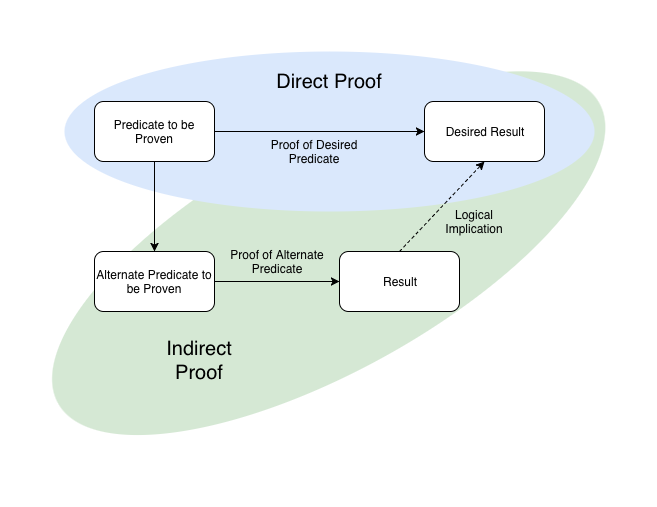
\includegraphics[scale=0.45]{res/direct_indirect.png}
		\caption{The algorithmic difference between the two types of proof structure.}
	\end{figure}	
	
	\newpage
	
	\section{``Induction"}
	We explore the definition of induction, and use it as motivation for the similarly named proof technique. \\
	
	% CITE
	According to Merriam-Webster, Induction is defined as: ``\emph{inference of a generalized conclusion from particular instances}." That is, the validity of a hypothesis is based on the breadth of cases for which said hypothesis does hold.\\
	
	An essential flaw of this type of induction is that one can never be \emph{totally} confident that a certain statement holds. For instance, it may be the case that no Beagle that has ever existed has never naturally grown green fur, but perhaps in the future there might exist a Beagle whose genetics are such that it does naturally grow green fur. In this way, one may be fairly confident in the statement \emph{``Beagles do not have green fur"}, but never totally confident. \\
	
	 In a similar vein, consider the predicate: $\forall n \in \mathbb{N}, n \geq 3, n^2 < 2^n$. Intuitively, this predicate seems true, and one could go about calculating the values for both $n^2$ and $2^n$, for $n = 1$ and then comparing those values to verify the predicate, repeating the process for $n=2$, then $n=3$, ... etc. However, the analogous problem presents itself here: what if there was some number $M \in \mathbb{N}$ that is beyond the scope of conceivable human (and computer) discovery\footnote{For example, Graham's Number}? How do we verify the predicate for such an unknown number?
	 
	\section{Induction}
		Induction is also known as a way to create the set $\mathbb{N}$. It is the following predicate: $$\text{If } n \in S, \text{ then } (n+1) \in S$$	
	\newpage
	
	\part{Questions}
		\begin{enumerate}
			\item Prove directly that the sum of an even integer and another even integer (not necessarily the same integer) is even.
				\subitem --- What can you conclude about the sum of an odd integer and an even integer? Can you directly prove it?
			\item \challenge Prove that any odd number is equal to a difference of squares\footnote{A difference of squares is of the form $(a^2 - b^2)$, where $a, b \in \mathbb{N}$}. 
				\subitem --- Hint: This difference of squares is not unique. 
				\subitem --- Hint: This proof is facilitated by \emph{constructing} the difference of squares.
			
			\item Prove $\sum_{i = 1}^{n} i^2 = \frac{n(n+1)(2n+1)}{6}$, by induction.
			\item Prove $\sum_{i = 1}^{n} i^3 = (\sum_{i = 1}^{n} i)^2 $.
			\item \challenge Prove, by induction that the degree-sum of the internal angles of $n$-sided polygon is equal to $(n-2)*180$:
				\begin{itemize}
					\item (\emph{Base Case}): What is the simplest shape for which this fact can be verified?
					% index = # sides, call it k?
					\item (\emph{Induction Hypothesis}): What may we use for our index value?
					\item (\emph{Induction Step}): Construct an arbitrary shape $S$, that has $k$ sides.
					\subitem{--- Argue there are 2 ways of creating a new side from an arbitrary side $s_i$ in $S$. Name this new shape $S\prime$.}
					\subitem{--- For each of the cases detailed above, verify that $S\prime$ satisfies the relevant angle equation, keeping in mind the number of 											sides in $S\prime$.}
				\end{itemize}
		\end{enumerate}
		
	
\end{document}